%%%%%%%%%%%%%%%%%%%%%%%%%%%%%%%%%%%%%%%%%%%%%%%%%%%%%%%%%%%%%%%%%
%_____________ ___    _____  __      __ 
%\____    /   |   \  /  _  \/  \    /  \  Institute of Applied
%  /     /    ~    \/  /_\  \   \/\/   /  Psychology
% /     /\    Y    /    |    \        /   Zuercher Hochschule 
%/_______ \___|_  /\____|__  /\__/\  /    fuer Angewandte Wissen.
%        \/     \/         \/      \/                           
%%%%%%%%%%%%%%%%%%%%%%%%%%%%%%%%%%%%%%%%%%%%%%%%%%%%%%%%%%%%%%%%%
%
% Project     : Seminararbeit
% Title       : 
% File        : anhang Rev. 00
% Date        : 10.10.2012
% Author      : Till J. Ernst
%
%%%%%%%%%%%%%%%%%%%%%%%%%%%%%%%%%%%%%%%%%%%%%%%%%%%%%%%%%%%%%%%%%

\pagenumbering{Roman}

\appendix
\chapter{Anhang}\label{chap.anhang}
\section{Glossar}\label{sec.glossar}
\begin{table}[ht] \centering
	%\caption{Klassifizierung}
	\begin{tabular}{b{4cm} m{11cm} }	
		\rowcolor{gray} 
		
		\textbf{Ausdruck} & \textbf{Definition} \\ 
		\textbf{Blog} & Kommt ursprünglich aus dem Wort 'Weblog', was soviel wie Webeintrag bedeutet und wurde eines Tages von einem Blogger (jemand der Einträge in Blogs vornimmt) ironischerweise in den Ausspruch 'we blog' (deutsch 'wir bloggen') umgewandelt. Seid diesem Zeitpunkt wird für diese Art von Web-Tagebuch das Wort Blog verwendet \cite{Kaplan:2012}.  \\ 
		\textbf{Tweet / Twitter} & Twitter gehört in die Kategorie 'Mikroblogging' und ermöglicht den Versand von telegrammartigen Kurznachrichten. Es handelt sich um ein Echtzeit-Informationsnetzwerk, welches die maximal 140 Zeichen langen Nachrichten ähnlich der Form eines Schneeballsystems versendet \cite{Twitter:2012}. \\ 
	
	\end{tabular}
	\label{tab:glossar}
\end{table}

\section{Grafik: Einfluss Subjektives Wohlbefinden}\label{sec.anhangGrafik}
\begin{figure}[H]
	\centering
		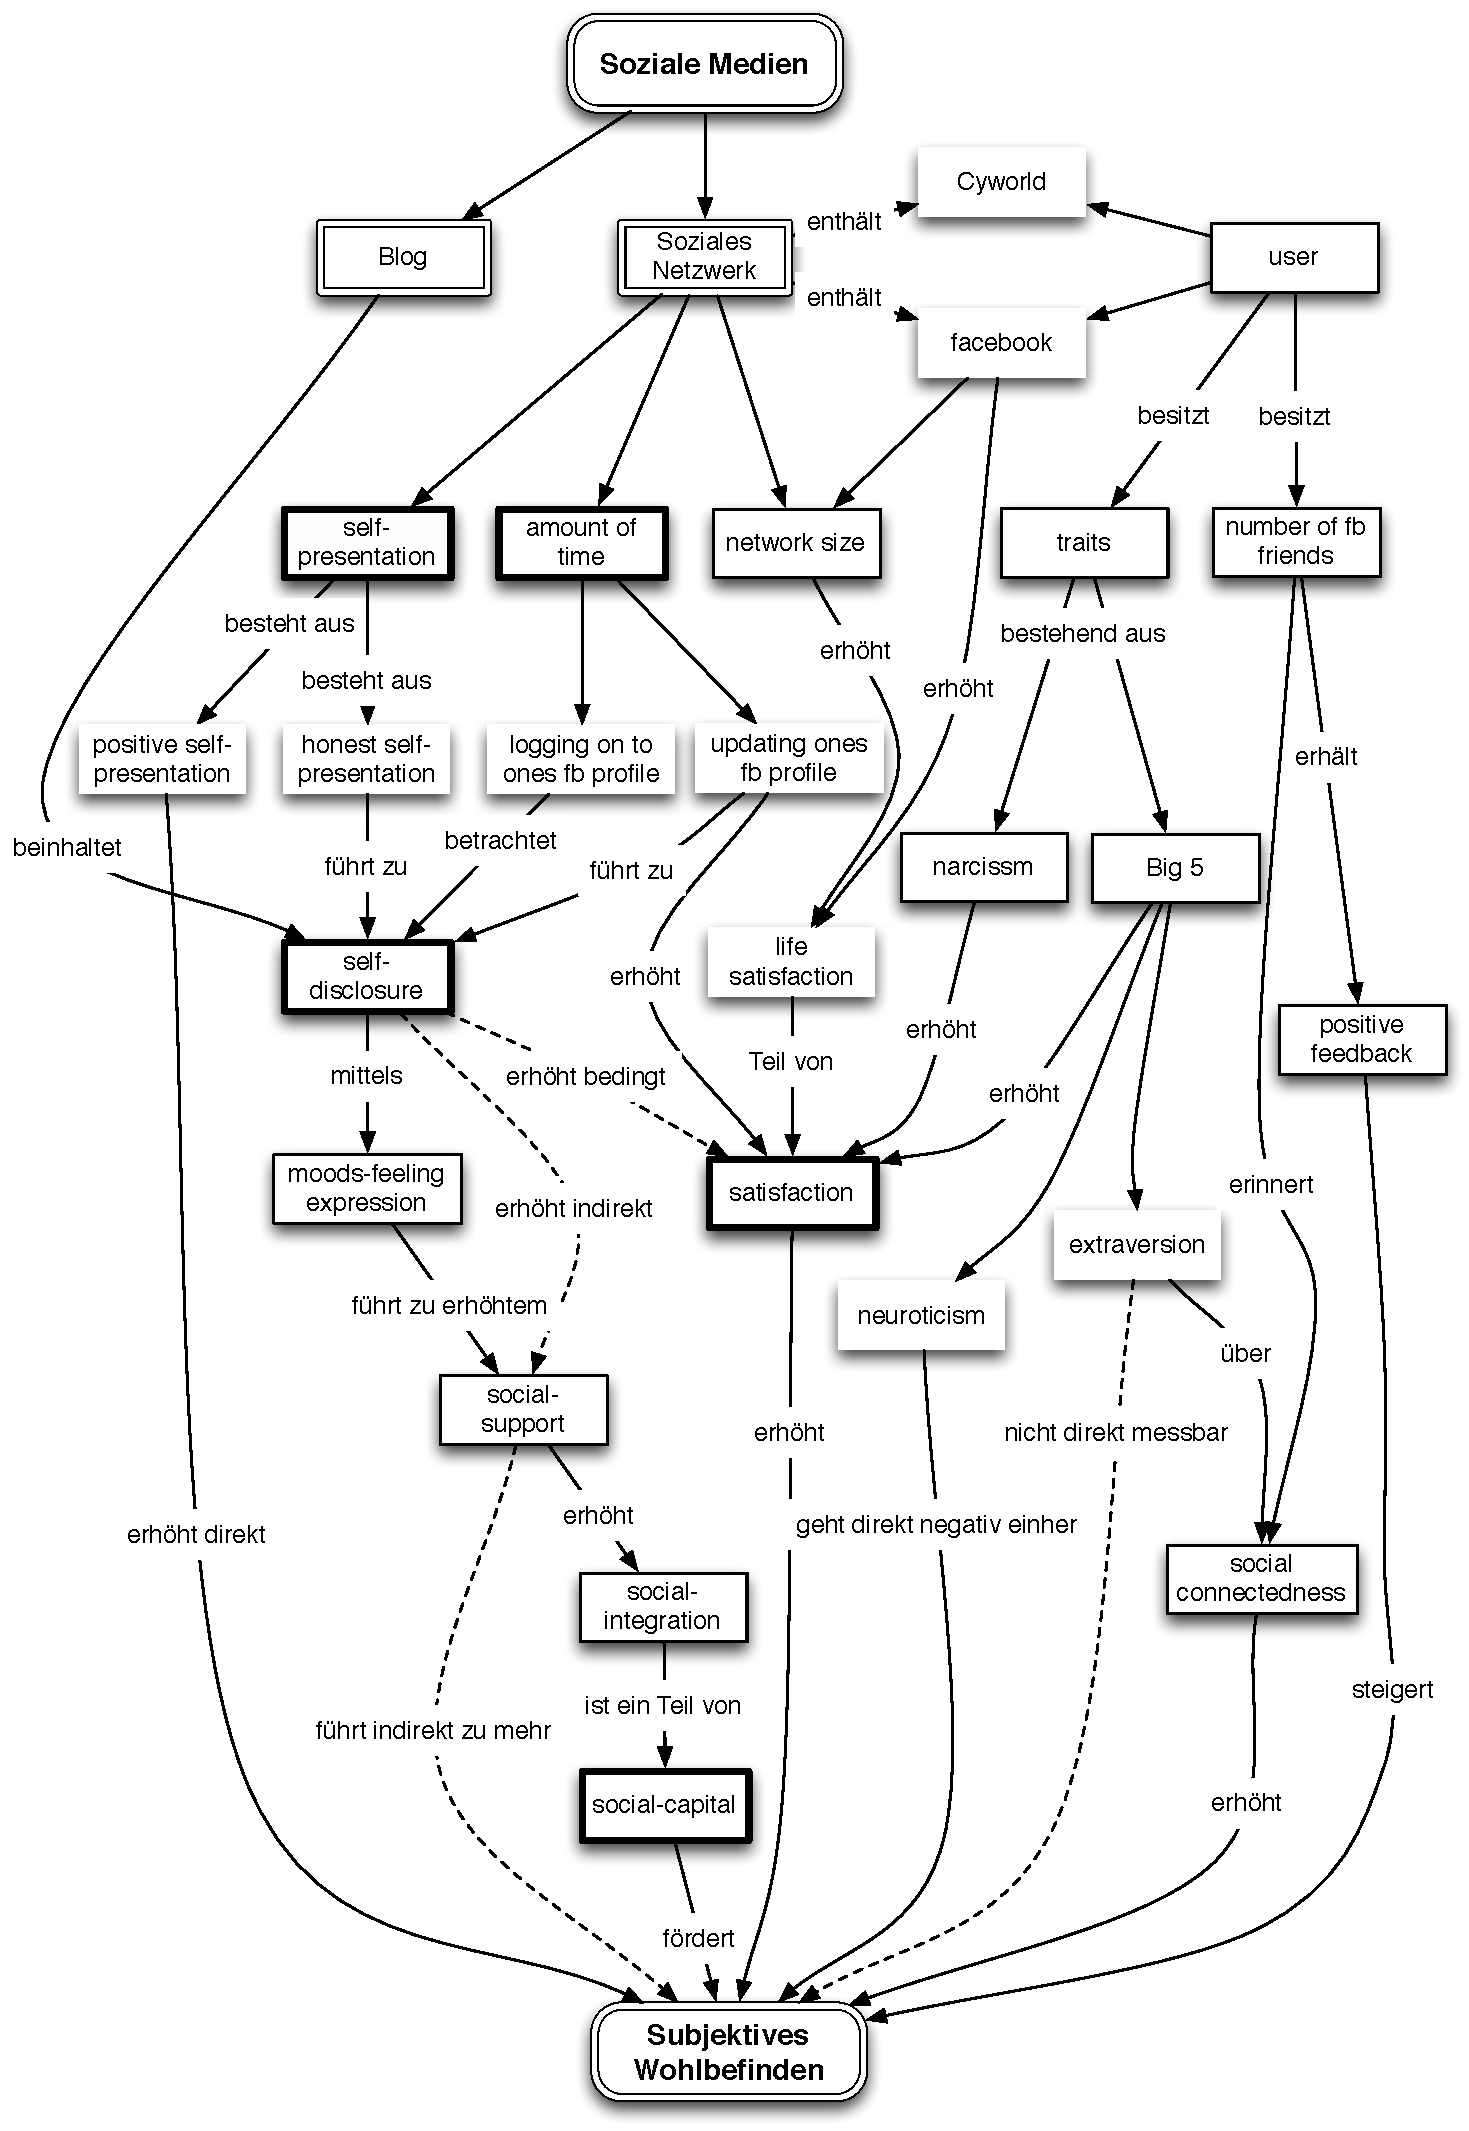
\includegraphics[width=0.9\textwidth]{images/grafiken/conceptMap_Swb_Sm_v2.pdf}
	\caption{ConceptMap - Subjektives Wohlbefinden und Soziale Medien}
	\label{fig.ConceptMapSwbSmAnhang}
\end{figure}
